\documentclass[twoside]{article} \usepackage{aistats2017}

% If your paper is accepted, change the options for the package
% aistats2017 as follows:
%
%\usepackage[accepted]{aistats2017}
%
% This option will print headings for the title of your paper and
% headings for the authors names, plus a copyright note at the end of
% the first column of the first page.

\bibliographystyle{apalike}  % Use the "unsrtnat" BibTeX style for formatting the Bibliography
\usepackage[square, authoryear, comma, sort&compress]{natbib}  % Use the "Natbib" style for the references in the Bibliography

\usepackage{amsmath}
\usepackage{amssymb}
\usepackage{amsthm}
\usepackage{mathbbol}
\usepackage{mathtools}
\usepackage{mathrsfs}
\usepackage{bm}
\usepackage{vector}
\usepackage[usenames, dvipsnames]{color}
\usepackage{cleveref}
\usepackage{graphicx}
\usepackage{caption}
\usepackage{subcaption}

\theoremstyle{definition}
\newtheorem{definition}{Definition}[section]
\theoremstyle{theorem}
\newtheorem{theorem}{Theorem}[section]
\newtheorem{corollary}{Corollary}[theorem]
\newtheorem{lemma}[theorem]{Lemma}

\newcommand{\argmin}{\operatornamewithlimits{argmin}}
\newcommand{\rv}[1]{{#1}}
\newcommand{\ds}[1]{\tilde{#1}}
\newcommand{\warn}[1]{{\color{red} #1}}
\newcommand{\extra}[1]{{\color{ForestGreen} #1}}
\newcommand{\qpi}{QPI}

\newcommand{\expect}[1]{{\mathbb{E}[#1]}}
\newcommand{\inner}[2]{{\langle #1, #2 \rangle}}

\newcommand{\Hk}{\mathcal{H}_{k}}
\newcommand{\Hl}{\mathcal{H}_{l}}
\newcommand{\muX}{\mu_{\rv{X}}}
\newcommand{\muY}{\mu_{\rv{Y}}}
\newcommand{\muYx}{\mu_{\rv{Y} | \rv{X} = x}}
\newcommand{\muXy}{\mu_{\rv{X} | \rv{Y} = y}}
\newcommand{\phiX}{\phi_{\rv{X}}}
\newcommand{\psiY}{\psi_{\rv{Y}}}
\newcommand{\Cxy}{C_{\rv{X} \rv{Y}}}
\newcommand{\Cyx}{C_{\rv{Y} \rv{X}}}
\newcommand{\Cxx}{C_{\rv{X} \rv{X}}}
\newcommand{\Cyy}{C_{\rv{Y} \rv{Y}}}
\newcommand{\Cylx}{C_{\rv{Y} | \rv{X}}}
\newcommand{\Cxly}{C_{\rv{X} | \rv{Y}}}

\newcommand{\hatmuX}{\hat{\mu}_{\rv{X}}}
\newcommand{\hatmuY}{\hat{\mu}_{\rv{Y}}}
\newcommand{\hatmuYx}{\hat{\mu}_{\rv{Y} | \rv{X} = x}}
\newcommand{\hatmuXy}{\hat{\mu}_{\rv{X} | \rv{Y} = y}}
\newcommand{\hatCxy}{\hat{C}_{\rv{X} \rv{Y}}}
\newcommand{\hatCyx}{\hat{C}_{\rv{Y} \rv{X}}}
\newcommand{\hatCxx}{\hat{C}_{\rv{X} \rv{X}}}
\newcommand{\hatCyy}{\hat{C}_{\rv{Y} \rv{Y}}}
\newcommand{\hatCylx}{\hat{C}_{\rv{Y} | \rv{X}}}
\newcommand{\hatCxly}{\hat{C}_{\rv{X} | \rv{Y}}}
\newcommand{\cardX}{\Vert \mathcal{X} \Vert}
\newcommand{\cardY}{\Vert \mathcal{Y} \Vert}

\begin{document}

% If your paper is accepted and the title of your paper is very long,
% the style will print as headings an error message. Use the following
% command to supply a shorter title of your paper so that it can be
% used as headings.
%
%\runningtitle{I use this title instead because the last one was very long}

% If your paper is accepted and the number of authors is large, the
% style will print as headings an error message. Use the following
% command to supply a shorter version of the authors names so that
% they can be used as headings (for example, use only the surnames)
%
%\runningauthor{Surname 1, Surname 2, Surname 3, ...., Surname n}

\twocolumn[

\aistatstitle{Nonparametric Quantile Regression with Kernel Embeddings}

\aistatsauthor{ Anonymous Author 1 \And Anonymous Author 2 \And Anonymous Author 3 }

\aistatsaddress{ Unknown Institution 1 \And Unknown Institution 2 \And Unknown Institution 3 } ]

\begin{abstract}

	Quantile regression is concerned with the estimation of quantiles from a conditional distribution of a response variable. This offers a more complete and robust inference framework than mean regression. This is especially important in decision making applications where a risk probability is used to bound the acceptable ranges of the response variable. In this paper, we develop a nonparametric quantile regression framework by utilising the expressive power and flexibility of kernel embedding models, which transforms probability distributions into unique mean embeddings that can be represented directly from data. We present a set of novel algorithms for computing quantiles from such a nonparametric inference model, and compare it to state-of-the-art algorithms in quantile regression. On multiple standard datasets, our methods produces competitive or improved quantile estimates in comparison to the literature.

\end{abstract}

\section{INTRODUCTION}
\label{sec:introduction}

	Understanding risk is critical in any discipline making decisions under uncertainty. Uncertainty can arise from both incomplete information and randomness in events, whose behaviour can be captured by probabilistic methods. In many cases, such decisions depend on one or more quantities of interest, where the likelihood that such quantities will fall outside a nominal or acceptable range is used to quantify the corresponding risks involved. For example, the material toughness of a motorcycle can be designed to withstand a likely range of acceleration experienced under collision, in order to limit the development cost. The probability that the actual acceleration experienced falls outside this nominal range is seen as the level of risk involved in this decision. 

	\begin{figure}
		\begin{center}
			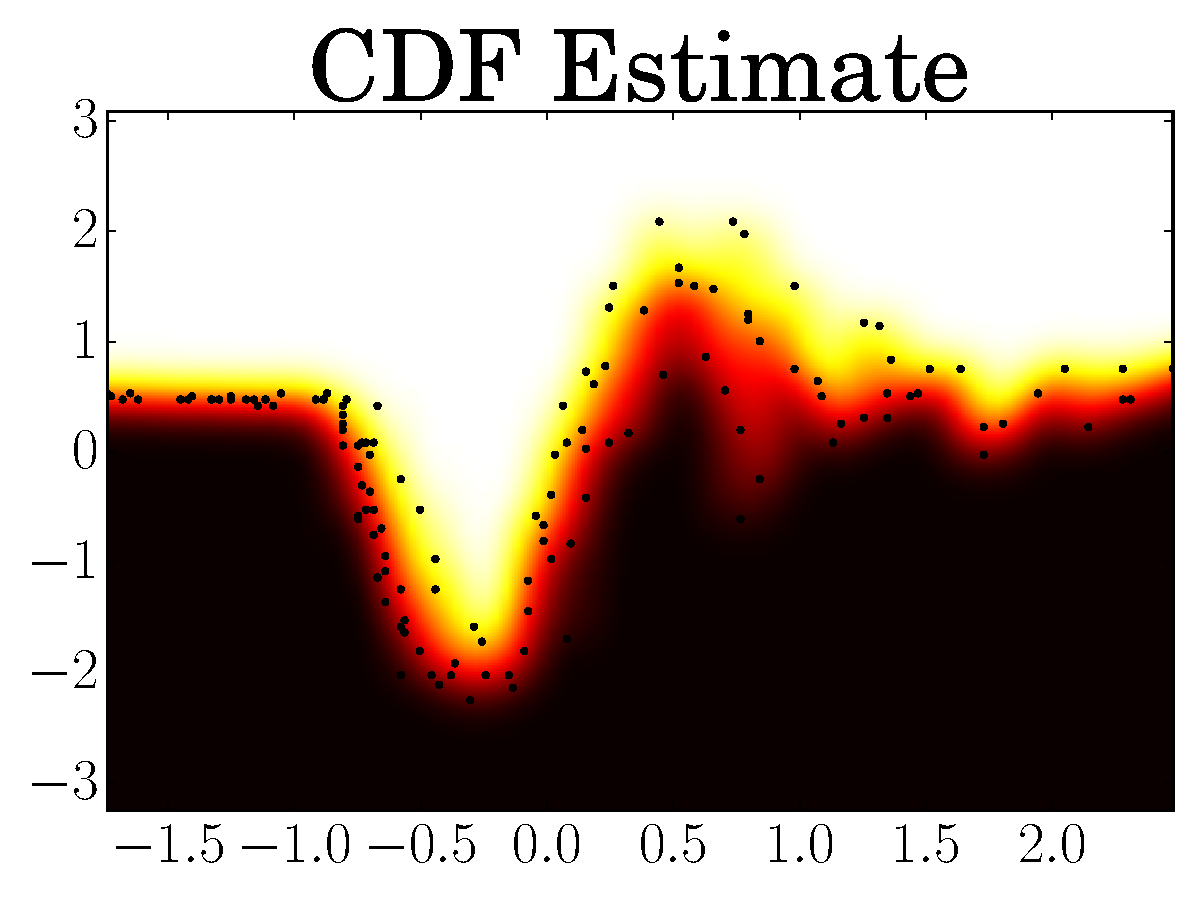
\includegraphics[width=0.48\columnwidth]{figures/mcquantiles_1}
			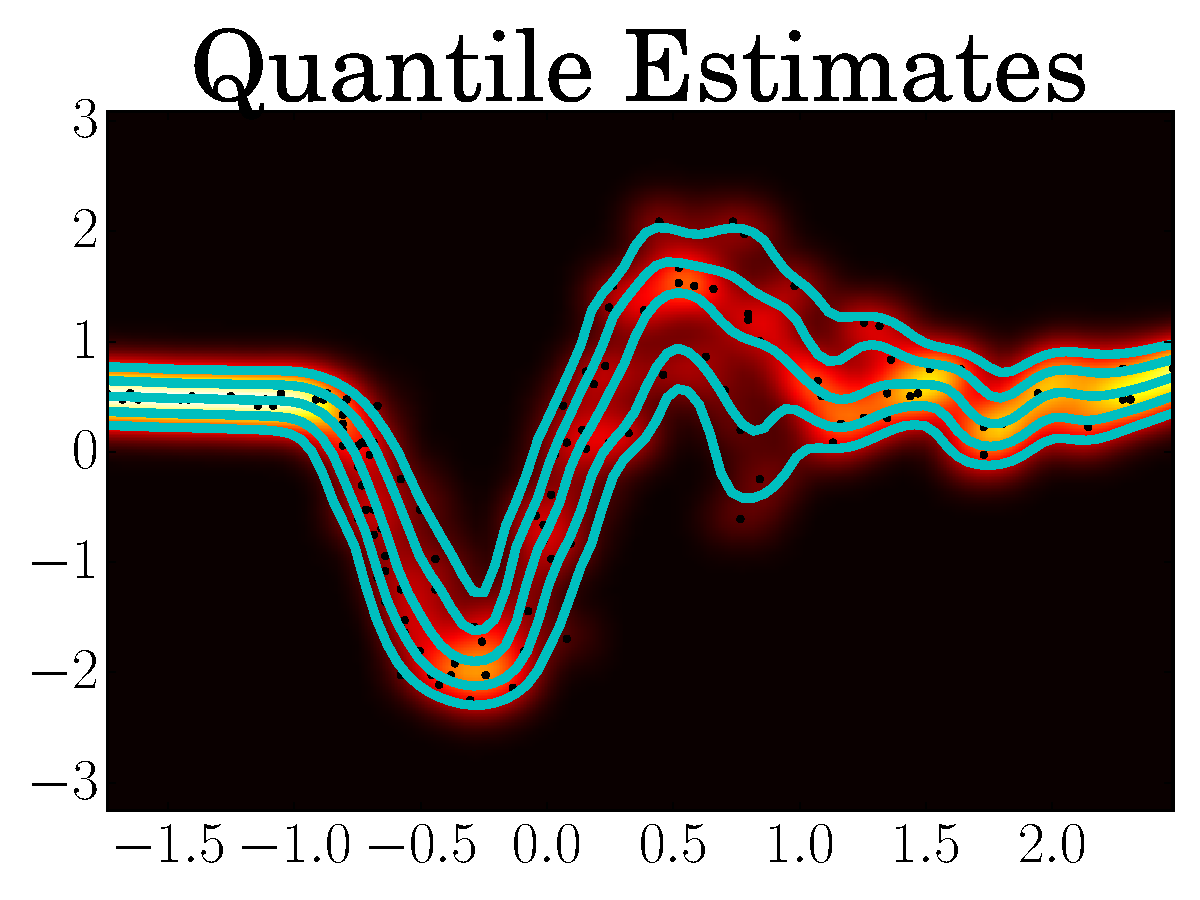
\includegraphics[width=0.48\columnwidth]{figures/mcquantiles_2}
		\end{center}
		\caption{\small CDF estimate (left), and the 0.1, 0.25, 0.5, 0.75, 0.9 quantiles overlaying a PDF estimate (right)} on a motorcycle dataset (acceleration v.s. time)
		\label{fig:quantile_regression_motorcycle}
	\end{figure}
	
	More naturally, however, instead of specifying an acceptable range of values and determining the level of risk involved, an acceptable risk probability can be specified instead, which is then used to obtain the bounds of the acceptable range. That is, we are interested in finding quantiles, which provide the bounds inside which a known mass of probability is contained. 
	
%	Bayesian methods in the machine learning community has demonstrated the advantages that probabilistic techniques bring forth. By maintaining not only a point estimate of a phenomenon, but a probability distribution of our belief about that phenomenon, informed decisions and actions can be taken by taking into account the uncertainty involved.
	
% * <lachlan@mccalman.info> 2016-10-05T23:30:52.467Z:
%
% These three sentences, whilst each good, could probably be made to connect more. Ie perhaps clarify the relationship between risk, uncertainty, decision making and Bayesian techniques?
% Done
% ^.

	When the quantity of interest is a response variable conditionally dependent on a input variable that is also continuous, the relationship can be captured by a regression model. \Cref{fig:quantile_regression_motorcycle} shows a typical example of quantile regression on motorcycle acceleration against time. Typically, the response variable is predicted with the mean, and the uncertainty of this prediction can be captured by the standard deviation. However, this is only natural in the case of an output phenomenon that is unimodal. Consider a bi-modal, symmetric distribution centred at zero with density peaks at $\pm1$ and a low density value at zero. The mean prediction of zero would not be a representative prediction of a likely sample or outcome, immediately also limiting the usefulness of the standard deviation which captures deviations from the mean. In this case, it is far more useful and natural to bound the uncertainty, or risk, through a quantile.
	
% * <lachlan@mccalman.info> 2016-10-05T23:33:18.326Z:
%
% Might be worth explicitly mentioning at the end here that a quantiles provide bounds inside which a known mass of probability is contained 
% Done
% ^.
	
%By embedding probability distributions as unique mean embeddings in a reproducing kernel Hilbert space, kernel embedding models reduce probabilistic marginalisation integrals into linear algebraic operations.

	In order to relax the unimodality restriction, we propose a set of novel quantile regression algorithms using kernel embedding techniques. By mapping general probability distributions into a reproducing kernel Hilbert space where marginalisation integrals become linear algebra operations, kernel embedding models are able to capture general, multimodal phenomenon. In this approach, probability distributions can be represented directly from data without assuming a parametric form, allowing quantile and risk inference on a variety of flexible distributions.
	
	In this paper, we present both \textit{direct} and \textit{pre-image} approaches. Direct approaches produces cumulative distribution estimates directly, and are thus more efficient in complexity. In contrast, pre-image approaches first recover the probability density beforehand, and are more accurate consequently. We derive several quantile regression methods based on these two approaches, using two learning schemes for hyperparameter optimisation. Finally, we demonstrate competitive or improved performance of our algorithms on standard datasets as compared to state-of-the-art algorithms in quantile regression from the literature.

% * <lachlan@mccalman.info> 2016-10-05T23:36:20.099Z:
% 
% rather than describing them as six algorithms, might be better to say 'a set of' or a series of or something, because they're all variations on a theme.
% Consider finding different words for 'letting the data speak for itself' -- it's a little colloquial
% Done!
% 
% ^.
	
\section{BACKGROUND}
\label{sec:background}
	
% * <lachlan@mccalman.info> 2016-10-05T23:47:01.875Z:
%
% I'd add a sentence at the beginning explaining that you're using the measure-theoretic notation (and possibly why)
% I mentioned that we are introducing notations from probability theory, which is a sub-field of measure theory.
%
% ^.
	We first introduce the necessary mathematical background and definitions. Let $(\Omega, \mathcal{W}, \mathbb{P})$ be a probability space, where $\Omega$ is the sample space, $\mathcal{W}$ is a $\sigma$-field on $\Omega$, and $\mathbb{P} : \mathcal{W} \to [0, 1]$ a probability measure. The elements $W$ of $\mathcal{W}$, that is, the measurable sets, are called events, which are by definition subsets of $\Omega$. Let $\mathcal{X}$ be some Borel measurable space of interest, endowed by a $\sigma$-field $\mathcal{A}$ on $\mathcal{X}$.
% * <lachlan@mccalman.info> 2016-10-05T23:45:45.159Z:
%
% I'd add a sentence here explaining why you're using the measure-theoretic approach.
% I would love to, but we are out of space. Maybe we will put this in the supplementary.
%
% ^ <lachlan@mccalman.info> 2016-10-05T23:46:46.888Z.
	
	\begin{definition} \label{def:distribution}
		\citep{bauer1981probability}
		The \textit{distribution} of a random variable $\rv{X} : \Omega \to \mathcal{X}$ is the Borel measure $\mathbb{P}_{\rv{X}} : \mathcal{A} \to [0, 1]$ defined by
		\begin{equation}
			\mathbb{P}_{\rv{X}}[A] := \mathbb{P}[\rv{X} \in A].
		\label{eq:distribution}
		\end{equation}
		where the event $\{\rv{X} \in A\} := \rv{X}^{-1}[A] := \{\omega \in \Omega : \rv{X}(\omega) \in A\} \in \mathcal{W}$ is the inverse image of $A \in \mathcal{A}$ (thus $A \subseteq \mathcal{X}$ by definition) under the random variable $\rv{X}$.
	\end{definition}
	
	\begin{definition} \label{def:cdf}
		\citep{bauer1981probability}
		The \textit{cumulative distribution function} (CDF) $P_{\bvec{\rv{X}}} : \mathbb{R}^{d} \to [0, 1]$ of a \textit{real-valued} random vector $\bvec{\rv{X}} : \Omega \to \mathbb{R}^{d}$ is
		
		\begin{equation}
				P_{\bvec{\rv{X}}}(\bvec{x}) := \mathbb{P}_{\bvec{\rv{X}}}[(-\bm{\infty}, \bvec{x}]] = \mathbb{P}[\bvec{\rv{X}} \leq \bvec{x}].
		\label{eq:cdf}
		\end{equation}

		For conciseness, we define the following shorthand \eqref{eq:shorthand},
		\begin{equation}
			\begin{aligned}
				\{\bvec{\rv{X}} \leq \bvec{x}\} &:= \bigcap\limits_{j = 1}^{d} \{\rv{X}_{j} \in (-\infty, x_{j}]\} \in \mathcal{W}, \\
				(-\bm{\infty}, \bvec{x}] &:= (-\infty, x_{1}] \times \dots \times (-\infty, x_{d}]. \\
			\end{aligned}
		\label{eq:shorthand}
		\end{equation}
	\end{definition}
		
	\subsection{Kernel Embedding}
	\label{sec:background:kernel_embedding}
	
%		This section summarises fundamental and important results in the field of kernel embeddings that form the background of this paper.

		In this paper we assume all kernels involved are positive definite and characteristic. A kernel $k : \mathcal{X} \times \mathcal{X} \to \mathbb{R}$ is \textit{characteristic} if it defines a unique reproducing kernel Hilbert space (RKHS), denoted by $\mathcal{H}_{k}$ \citep{fukumizu2004dimensionality}. Let $\rv{X} : \Omega \to \mathcal{X}$ and $\rv{Y} : \Omega \to \mathcal{Y}$ be random variables with distributions $\mathbb{P}_{\rv{X}}$ and $\mathbb{P}_{\rv{Y}}$, and let $k$ and $l$ be characteristic positive definite kernels defined on $\mathcal{X}$ and $\mathcal{Y}$ respectively. Let $f \in \Hk$ and $g \in \Hl$ be real-valued functions.
		
		The feature function of a RKHS can be obtained from the partially applied kernels $\phi_{x} := k(x, \cdot) \in \Hk$ and $\psi_{y} := l(y, \cdot) \in \Hl$, and forms the basis for the full RKHS. An inner product in the RKHS satisfies the reproducing property \eqref{eq:reproducing_property}, where the function evaluation operator within the full RKHS is the inner product with the feature function \citep{muandet2016kernel},
		\begin{equation}
			\inner{\phi_{x}}{f} = f(x) ,\quad \inner{\psi_{y}}{g} = g(y).
		\label{eq:reproducing_property}
		\end{equation}
		
%		\extra{
%		In particular, the kernel value between two points can be evaluated as the inner product between the feature functions at those points \eqref{eq:kernel_reproducing_property}.
%
%		\begin{equation}
%			\inner{\phi_{x}}{\phi_{x'}} = k(x, x') ;\quad \inner{\psi_{y}}{\psi_{y'}} = l(y, y')
%		\label{eq:kernel_reproducing_property}
%		\end{equation}
%		}
		
		\begin{definition} \label{def:kernel_embedding}
			\citep{smola2007hilbert}
			The \textit{kernel embedding} (or \textit{mean embedding}) of a distribution $\mathbb{P}_{\rv{X}}$ is defined as the expectation of the corresponding feature function in that RKHS \eqref{eq:kernel_embedding},
			\begin{equation}
				\muX \equiv \muX(\cdot) := \expect{\phiX} = \expect{k(\rv{X}, \cdot)} \in \Hk.
			\label{eq:kernel_embedding}
			\end{equation}
		\end{definition}
		
		Kernel embeddings are powerful tools as each embedding $\muX$ holds all the statistical information of its corresponding distribution $\mathbb{P}_{\rv{X}}$, and this correspondence is unique for a characteristic kernel $k$. Furthermore, expectations of a function in the RKHS can be evaluated as the inner product \eqref{eq:function_expectation} between the kernel embedding and the function \citep{muandet2016kernel},
		\begin{equation}
			\inner{\muX}{f} = \expect{f(\rv{X})} ,\quad \inner{\muY}{g} = \expect{g(\rv{Y})}.
		\label{eq:function_expectation}
		\end{equation}

		
		\subsubsection{Empirical Representation}
		\label{sec:background:kernel_embeddings:empirical_representation}
			
			In practice, the actual probability distributions of interest are not available in closed form, so that the mean embedding \eqref{eq:kernel_embedding} cannot be directly computed. Instead, independent and identically distributed (\textit{iid}) samples from probability distributions are available. Suppose that joint samples $\{x_{i}, y_{i}\}_{i = 1}^{n}$ are observed and collected in an \textit{iid} fashion from the joint distribution $\mathbb{P}_{\rv{X} \rv{Y}}$. Let $\ds{X} := \{x_{i}\}_{i = 1}^{n}$ and $\ds{Y} := \{y_{i}\}_{i = 1}^{n}$. It is possible to represent kernel embeddings empirically such that in the limit of infinite data, the empirical representations would converge to the true representations at an appropriate rate. Most significant, however, is the fact that important results for manipulating kernel embeddings also hold for their empirical representations \citep{muandet2016kernel}.
			
			By replacing the expectation with an empirical average, the resulting estimator \eqref{eq:empirical_embedding} converges to the true embedding \eqref{eq:kernel_embedding} at rate $O(n^{-1/2})$ \citep{smola2007hilbert},
			\begin{equation}
				\hatmuX := \frac{1}{n} \sum_{i = 1}^{n} \phi_{x_{i}} ,\quad \hatmuY := \frac{1}{n} \sum_{i = 1}^{n} \psi_{y_{i}}.
			\label{eq:empirical_embedding}
			\end{equation}

%			Correspondingly, the empirical representation of a function expectation is simply the empirical average of the function, and can be obtained by the inner product of the function with the empirical embedding \eqref{eq:empirical_function_expectation}.
%
%			\begin{equation}
%				\inner{\hatmuX}{f} = \frac{1}{n} \sum_{i = 1}^{n} f(x_{i}) ;\quad \inner{\hatmuY}{g} = \frac{1}{n} \sum_{i = 1}^{n} g(y_{i})
%			\label{eq:empirical_function_expectation}
%			\end{equation}

		
%			Since the samples $\ds{X} := \{x_{i}\}_{i = 1}^{n}$ and $\ds{Y} := \{y_{i}\}_{i = 1}^{n}$ are sampled from the joint distribution $\mathbb{P}_{\rv{X} \rv{Y}}$ such that marginal samples are simply $\ds{X}$ and $\ds{Y}$ themselves, the empirical representations for regular embeddings $\muX$ and $\muY$ are easy to obtain, as per \cref{thm:empirical_embedding}.
%			
%			However, instead of a uniform average, a empirical representations of the conditional embedding would require a weighted average of the following sform \eqref{eq:empirical_conditional_embedding_form} instead.
%			
%			\begin{equation}
%			\begin{aligned}
%			\hatmuYx &= \sum_{i = 1}^{n} \alpha_{i} \psi_{y_{i}} ;\quad \hatmuXy &= \sum_{i = 1}^{n} \beta_{i} \phi_{x_{i}}
%			\label{eq:empirical_conditional_embedding_form}
%			\end{aligned}
%			\end{equation}
%			
%			where $\bm{\alpha} := \{\alpha_{i}\}_{i = 1}^{n}$ is to be determined from the samples $\ds{X}$ and $\bm{\beta} := \{\beta_{i}\}_{i = 1}^{n}$ is to be determined from the samples $\ds{Y}$.
%			
%			Before deriving the expressions for $\bm{\alpha}$ and $\bm{\beta}$ however, it is useful to introduce matrix notation for representing empirical embeddings.
%			
%			The feature functions can be viewed as an feature vector of the same dimension as the cardinality of the its domain. For example, if the domain $\mathcal{X} = \mathbb{R}^{d}$ is the $d$ dimensional euclidean space whose cardinality is uncountably infinite, then the feature function can be viewed as an uncountably infinite dimensional feature vector, indexed by the elements of $\mathcal{X} = \mathbb{R}^{d}$.
%			
%			Denote the cardinality of $\mathcal{X}$ as $\cardX$, and similarly the cardinality of $\mathcal{Y}$ as $\cardY$. With the observations $\{x_{i}, y_{i}\}_{i = 1}^{n}$ sampled from $\mathbb{P}_{\rv{X} \rv{Y}}$, there are $n$ feature vectors for each RKHS, $\{\phi_{x_{i}}\}_{i = 1}^{n}$ for $\Hk$ and $\{\psi_{y_{i}}\}_{i = 1}^{n}$ for $\Hl$. As elements within their respective RKHS for which Hilbert-Schmidt operators can operate on, $\phi_{x_{i}}$ has an effective dimension of $\cardX \times 1$ and $\psi_{y_{i}}$ has an effective dimension of $\cardY \times 1$. Since this can be said about the feature functions, which form the basis for the RKHS, this also applies to general functions within the RKHS. As such, the inner product between functions $f_{1}, f_{2} \in \Hk$ can also be written in matrix notation as $\inner{f_{1}}{f_{2}} = f_{1}^{T} f_{2}$. It can be conceptually helpful to check that $f_{1}^{T}$ is of size $1 \times \cardX$ and $f_{2}$ is of size $\cardX \times 1$ so that the result is a scalar of size $1 \times 1$.
%			
%			Recall that a matrix $A := \begin{bmatrix} \bvec{a}_{1} & \cdots & \bvec{a}_{n} \end{bmatrix} \in \mathbb{R}^{n \times n}$, $\bvec{a}_{i} \in \mathbb{R}^{n} \; \forall i \in \{1, \dots, n\}$, operated on a vector $\bvec{v} \in \mathbb{R}^{n}$ results in a vector that is the linear combination of the columns of $A$ with coefficients given by the components of $\bvec{v}$. That is, $A \bvec{v} = \sum_{i = 1}^{n} v_{i} \bvec{a}_{i}$.
%			
%			Similarly, a feature matrix can be defined in the same way such that empirical representations of kernel embeddings can be reduced down to linear algebraic operations.
%			
			Following the notation of \cite{muandet2016kernel}, a feature matrix $\Phi \equiv \Phi_{\ds{X}}$ is formed by stacking the corresponding feature functions \textit{horizontally} \eqref{eq:feature_matrix}, where each function represents a column of that matrix,	
			\begin{equation}
				\Phi := \begin{bmatrix} \phi_{x_{1}} & \cdots & \phi_{x_{n}} \end{bmatrix}, \; \Psi := \begin{bmatrix} \psi_{y_{1}} & \cdots & \psi_{y_{n}} \end{bmatrix}.
			\label{eq:feature_matrix}
			\end{equation}
			The subscripts of $\Phi$ and $\Psi$ are dropped whenever it is clear from context the dataset involved. In this way, $\Phi$ and $\Psi$ has effective size $\cardX \times n$ and $\cardY \times n$, where $\Vert \cdot \Vert$ denotes the cardinality of a set, which is uncountably infinite in the case for continuous Euclidean spaces.
			
			With this notation, general empirical embeddings can then be expressed as the matrix product of a feature matrix and a weight vector of size $n \times 1$ \eqref{eq:empirical_conditional_embedding_matrices},
			\begin{equation}
			\hatmuXy = \sum_{i = 1}^{n} \beta_{i} \phi_{x_{i}} = \Phi \bm{\beta} ,\quad \hatmuYx = \Psi \bm{\gamma}.
			\label{eq:empirical_conditional_embedding_matrices}
			\end{equation}			
			where $\bm{\gamma} := \{\gamma_{i}\}_{i = 1}^{n}$ depends on $\ds{X}$ and $\bm{\beta} := \{\beta_{i}\}_{i = 1}^{n}$ depends on $\ds{Y}$ for a conditional embedding. For marginal embeddings, the weights become uniform such that $\gamma_{i} = \frac{1}{n}$ and $\beta_{i} = \frac{1}{n}$ for $i \in \{1, \dots, n\}$. However, the marginal embeddings will be written with general weights in later sections, as our technique can be applied to any embedding in general.

	\subsection{Quantiles and Quantile Regression}
	\label{sec:background:quantiles}

		At the heart of quantile regression is the quantile itself, which bounds the probability mass of a distribution.
		\begin{definition} \label{def:quantile}
			\citep{takeuchi2006nonparametric}
			Consider a real-valued random variable $\rv{X} : \Omega \to \mathbb{R}$. The \textit{$\tau$-quantiles}, $\tau \in (0, 1)$, of $\mathbb{P}_{\rv{X}}$ is the smallest value $x$ for which the CDF is still an upper bound for $\tau$,
			\begin{equation}
				q_{\rv{X}}(\tau) := \inf\{x : P_{\rv{X}}(x) \geq \tau\} \equiv \inf_{P_{\rv{X}}(x) \geq \tau} x.
			\label{eq:quantile}
			\end{equation}
%			\begin{equation}
%				\begin{aligned}
%					q_{\rv{X}}(\tau) &:= \inf\{x : P_{\rv{X}}(x) \geq \tau\} \equiv \inf_{P_{\rv{X}}(x) \geq \tau} x \\
%					q_{\rv{X} | \bvec{\rv{Y}} = \bvec{y}}(\tau) &:= \inf\{x : P_{\rv{X} | \bvec{\rv{Y}} = \bvec{y}}(x) \geq \tau\} \equiv \inf_{P_{\rv{X} | \bvec{\rv{Y}} = \bvec{y}}(x) \geq \tau} x
%				\end{aligned}
%			\label{eq:quantile}
%			\end{equation}
		\end{definition}
		Finding the conditional quantile $q_{\rv{X} | \bvec{\rv{Y}}}(\tau)$ is an identical problem to finding a regular quantile $q_{\rv{X}}(\tau)$, except with the CDF $P_{\rv{X}}$ replaced by a conditional CDF $P_{\rv{X} | \bvec{\rv{Y}} = \bvec{y}}$. For brevity, we will present CDF estimation from an embedding with general weights, whose form is shared by both conditional and regular embeddings.

		Quantile regression is then the problem of finding an empirical estimate $\hat{q}_{\rv{X} | \bvec{\rv{Y}} = \bvec{y}}(\tau)$ for $q_{\rv{X} | \bvec{\rv{Y}} = \bvec{y}}(\tau)$ given observations $\{(\bvec{y}_{i}, x_{i})\}_{i = 1}^{n}$ and a query point $\bvec{y}$.
		
		In practice, the infimum is often replaced with the minimum. If the CDF estimate is smooth and always increasing, the inequality becomes an equality, and obtaining quantiles becomes a root finding procedure once an estimate of the CDF is obtained \eqref{eq:quantile_root_finding},
		\begin{equation}
			q_{\rv{X}}(\tau) = x : P_{\rv{X}}(x) = \tau.
		\label{eq:quantile_root_finding}
		\end{equation}	
		Therefore, in this paper, we focus on techniques for CDF estimation from a given dataset, using both direct and pre-image approaches.
	
\section{DIRECT QUANTILE REGRESSION}
\label{sec:direct_quantile_regression}

	The direct approach to quantile regression refers to techniques which computes an estimate of the CDF directly, without needing to compute the PDF first.
	
	Using \eqref{eq:function_expectation}, our approach begins by expressing the distribution as an inner product between the mean embedding and the indicator function \eqref{eq:distribution_inner}, 
	\begin{equation}
		\mathbb{P}_{\bvec{\rv{X}}}[A] = \expect{\mathbb{1}_{A}(\bvec{\rv{X}})} = \inner{\mu_{\bvec{\rv{X}}}}{\mathbb{1}_{A}}.
	\label{eq:distribution_inner}
	\end{equation}
	The CDF  $P_{\bvec{\rv{X}}}$ reveals a similar structure to the distribution $\mathbb{P}_{\rv{X}}$ through \cref{def:cdf} \eqref{eq:cdf_inner},	
	\begin{equation}
		P_{\bvec{\rv{X}}}(\bvec{x}) := \mathbb{P}_{\bvec{\rv{X}}}[(-\bm{\infty}, \bvec{x}]] = \inner{\mu_{\bvec{\rv{X}}}}{\mathbb{1}_{(-\bm{\infty}, \bvec{x}]}}.
	\label{eq:cdf_inner}
	\end{equation}
	We will now focus our attention on how to estimate the distribution and CDF from a given dataset by empirically estimating \eqref{eq:distribution_inner} and \eqref{eq:cdf_inner}.
	
	\subsection{Optimal Function Projection}
	\label{sec:direct_quantile_regression:optimal_function_approximation}
	
		In order to estimate the distribution and CDF empirically, we would need both the empirical kernel embedding $\hat{\mu}_{\bvec{\rv{X}}}$ and a projection $\hat{\mathbb{1}}_{A}$ of the indicator function $\mathbb{1}_{A}$ into the same RKHS as $\hat{\mu}_{\bvec{\rv{X}}}$ so that a proper inner product within that RKHS can be evaluated.

		Suppose $\ds{X} := \{\bvec{x}_{1}, \dots, \bvec{x}_{n}\} \in \mathbb{R}^{n \times d}$ is set of observations from $\mathbb{P}_{\rv{X}}$. Functions that can be represented by these samples are linear combinations of the feature functions $\phi_{\bvec{x}_{i}}$ \eqref{eq:function_projection} \citep{muandet2016kernel},
		\begin{equation}
			\hat{f} = \sum_{i = 1}^{n} \alpha_{i} k(\bvec{x}_{i}, \cdot) = \sum_{i = 1}^{n} \alpha_{i} \phi_{\bvec{x}_{i}} = \Phi \bm{\alpha}.
		\label{eq:function_projection}
		\end{equation}
		The span obtained by those basis $\{\phi_{\bvec{x}_{i}}\}_{i = 1}^{n}$ also forms a RKHS, denoted by $\mathcal{H}_{k, \ds{X}}$, and is a finite vector subspace of the full RKHS $\mathcal{H}_{k}$.

		We are interested in approximating $f \in \mathcal{H}_{k}$ with $\hat{f} \in \mathcal{H}_{k, \ds{X}}$ through tuning the weights \eqref{eq:function_projection_optimisation} until they are closest as measured by the RKHS-induced norm \eqref{eq:function_projection_optimisation},
		\begin{equation}
			\bm{\alpha}^{\star} = \argmin_{\bm{\alpha} \in \mathbb{R}^{n}} \Vert \hat{f} - f \Vert.
		\label{eq:function_projection_optimisation}
		\end{equation}
		This optimisation has a solution given by \cref{thm:function_projection_solution}.
		\begin{theorem} \label{thm:function_projection_solution}
			The optimisation \eqref{eq:function_projection_optimisation} has a closed form solution $\bm{\alpha}^{\star} = K^{-1} \bvec{f}$ \eqref{eq:function_projection_solution}, where $K \equiv K_{\ds{X} \ds{X}} := \{k(\bvec{x}_{i}, \bvec{x}_{j})\}_{i = 1, j = 1}^{n, n}$ is the gram matrix and $\bvec{f} := f\{\ds{X}\} := \{f(\bvec{x}_{i})\}_{i = 1}^{n}$,
			\begin{equation}
				\hat{f} = \Phi \bm{\alpha}^{\star} = \Phi K^{-1} \bvec{f}.
			\label{eq:function_projection_solution}
			\end{equation}
		\end{theorem}
		The proof is given in the supplementary material.

	\subsection{Direct Empirical Distribution}
	\label{sec:direct_quantile_regression:optimal_empirical_distribution}
	
		If $\mathbb{1}_{A} \in \mathcal{H}_{k}$, we can let $f = \mathbb{1}_{A}$ and project it into $\mathcal{H}_{k, \ds{X}}$ as $\hat{\mathbb{1}}_{A} = \Phi K^{-1} \mathbb{1}_{A}\{\ds{X}\}$ using \cref{thm:function_projection_solution}. Motivated by \eqref{eq:distribution_inner}, \cref{thm:empirical_distribution_and_cdf} provides a direct distribution and CDF estimate. The derivation is given in the supplementary material.
		\begin{theorem} \label{thm:empirical_distribution_and_cdf}
			Assume that a kernel $k$ is chosen such that the indicator function is in $\mathcal{H}_{k}$. The direct empirical distribution measured on a set is simply the sum of weights on that set \eqref{eq:empirical_distribution},
			\begin{equation}
				\hat{\mathbb{P}}_{\bvec{\rv{X}}}[A] := \inner{\hat{\mu}_{\bvec{\rv{X}}}}{ \hat{\mathbb{1}}_{A}} = \sum_{i : \bvec{x}_{i} \in A} \beta_{i}.
			\label{eq:empirical_distribution}
			\end{equation}
			By \cref{def:cdf}, the CDF shows a similar form \eqref{eq:empirical_cdf},
			\begin{equation}
				\hat{P}_{\bvec{\rv{X}}}(\bvec{x}) := \hat{\mathbb{P}}_{\bvec{\rv{X}}}[(-\bm{\infty}, \bvec{x}]] = \sum_{i : \bvec{x}_{i} \leq \bvec{x}} \beta_{i}.
			\label{eq:empirical_cdf}
			\end{equation}
		\end{theorem}
		Nevertheless, in order to apply \cref{thm:empirical_distribution_and_cdf}, the class of applicable kernels is restricted to those whose RKHS $\mathcal{H}_{k}$ contains the indicator function. \cite{kanagawa2014recovering} showed that the estimator $\langle \hat{\mu}_{\bvec{\rv{X}}}, \hat{f} \rangle$ is consistent for $\mathbb{E}[f(\bvec{\rv{X}})]$ if $f$ is in the Besov space, which is a superset of the full RKHS $\mathcal{H}_{k}$. This means that \cref{thm:empirical_distribution_and_cdf} also holds if the indicator function is in the Besov space. However, experiments show that even if this assumption is not satisfied, the estimators provided in \cref{thm:empirical_distribution_and_cdf} still converges to the true distribution and CDF empirically.

	\subsection{Smooth Empirical Distribution}
	\label{sec:direct_quantile_regression:smooth_empirical_distribution}

		\begin{figure}
			\begin{center}
				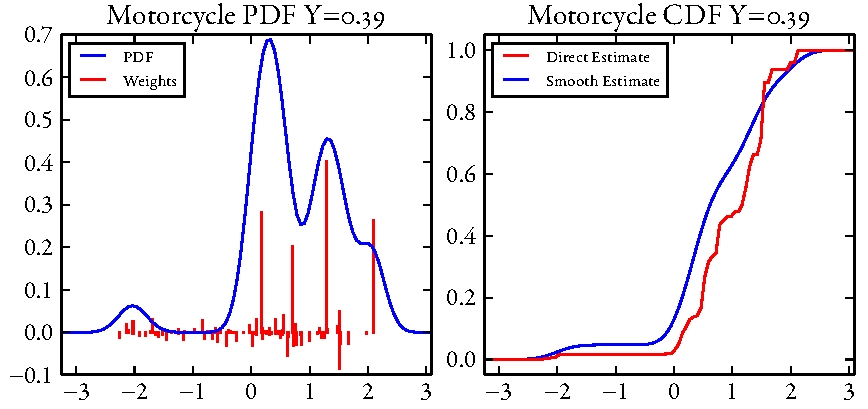
\includegraphics[width=\columnwidth]{figures/cumulativeexamplesmooth}
				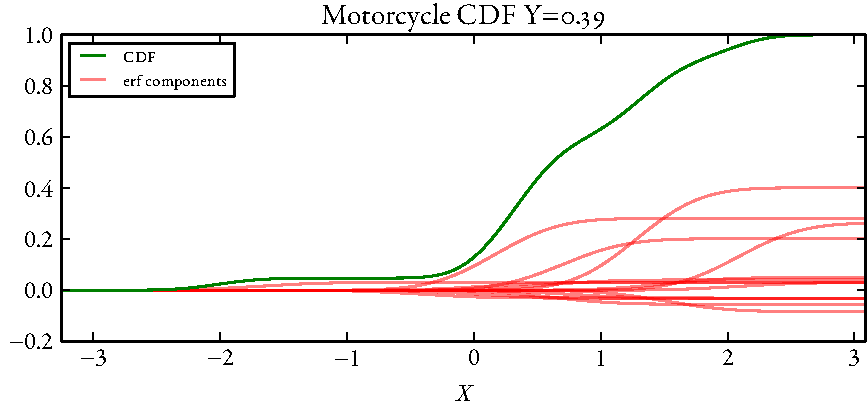
\includegraphics[width=\columnwidth]{figures/cumulativeexampleerf}
			\end{center}
			\caption{\small (Left) The PDF obtained through the pre-image method on the Motorcycle dataset (blue) and The embedding weights at the training points (red). (Right) The resulting CDF estimate using the direct estimate \eqref{eq:empirical_cdf} and smooth estimate \eqref{eq:smooth_empirical_cdf_gaussian_kernel}. (Bottom) The smooth CDF estimate again (green) with its individual error function components (red) overlayed \eqref{eq:smooth_empirical_cdf_gaussian_kernel}.}
			\label{fig:direct_quantile_regression}
		\end{figure}
		
		By embedding indicator functions, the resulting CDF estimate \eqref{eq:empirical_cdf} is discontinuous at the jumps located at each data point. Directly differentiating this would result in a superposition of Dirac deltas for the PDF. However, in many applications, the PDF is rather smooth, and thus so is the CDF. Many characteristic kernels are also smooth, and thus so are the functions within their RKHS. Therefore, instead of taking the inner product with the indicator projection $\hat{1}_{A}$ into $\mathcal{H}_{k, \ds{X}}$, we propose to take the inner product with the indicator projection $\tilde{1}_{A}$ into the full RKHS $\mathcal{H}_{k}$ \eqref{eq:indicator_smooth},
		\begin{equation}
			\tilde{\mathbb{1}}_{A} := \int_{\mathcal{X}} \mathbb{1}_{A}(\bvec{x}) k(\bvec{x}, \cdot) d\bvec{x} = \int_{A} k(\bvec{x}, \cdot) d\bvec{x},
		\label{eq:indicator_smooth}
		\end{equation}
		which would converges to the indicator function $\mathbb{1}_{A}$ as the kernel bandwidth goes to zero. This leads to the following smooth distribution and CDF estimate. The derivation is given in the supplementary material.
		\begin{theorem} \label{thm:smooth_empirical_distribution_and_cdf}
			The smooth distribution estimate \eqref{eq:smooth_empirical_distribution},
			\begin{equation}
				\hat{\mathbb{P}}_{\bvec{\rv{X}}}[A] := \inner{\hat{\mu}_{\bvec{\rv{X}}}}{\tilde{\mathbb{1}}_{A}} = \sum_{i = 1}^{n} \beta_{i} \int_{A}  k(\bvec{x}_{i}, \bvec{x}) d\bvec{x},
			\label{eq:smooth_empirical_distribution}
			\end{equation}
			and the smooth CDF estimate \eqref{eq:smooth_empirical_cdf},
			\begin{equation}
				\hat{P}_{\bvec{\rv{X}}}(\bvec{x}) = \sum_{i = 1}^{n} \beta_{i} \int_{-\bm{\infty}}^{\bvec{x}}  k(\bvec{x}_{i}, \bvec{x}') d\bvec{x}' = \bm{\beta}^{T} \bvec{K}(\bvec{x}),
			\label{eq:smooth_empirical_cdf}
			\end{equation}
			can be obtained by integrating the corresponding mean embedding, resulting in a linear combination of kernel integrals. The vector of kernel integrals is notated by
			\begin{equation}
				\bvec{K}(\bvec{x}) := \Bigg\{ \int_{-\bm{\infty}}^{\bvec{x}}  k(\bvec{x}_{i}, \bvec{x}') d\bvec{x}' \Bigg\}_{i = 1}^{n}.
			\label{eq:kernel_integral}
			\end{equation}
		\end{theorem}
		The estimates are expressed as a summation of the kernel integrals, which would need to be analytically derived or otherwise estimated. For a Gaussian kernel, analytical form can be derived \eqref{eq:smooth_empirical_cdf_gaussian_kernel},
		\begin{equation}
			\hat{P}_{\bvec{\rv{X}}}(\bvec{x}) = \frac{1}{2} \sum_{i = 1}^{n} \beta_{i} \prod_{j = 1}^{d} \Bigg[1 + \mathrm{erf}\bigg(\frac{x_{j} - x_{i, j}}{\sigma_{j} \sqrt{2}}\bigg)\Bigg].
		\label{eq:smooth_empirical_cdf_gaussian_kernel}
		\end{equation}
		Even if the analytical form cannot be derived for some kernels $k$, since it is independent of the embedding weights, the integral $\bvec{K}(\bvec{x}) \equiv \bvec{K}_{\ds{X}}(\bvec{x})$ \eqref{eq:kernel_integral} can be approximated and pre-computed before inference begins.

		With this approach, CDF estimates are now smooth and can be shown to converge to the true CDF in the limit of $n \rightarrow \infty$ and vanishing kernel bandwidth. However, due to the possibility of negative weights $\beta_{i}$, both direct approaches may produce CDF estimates that are not strictly non-decreasing, as shown in \cref{fig:direct_quantile_regression}. Notice that the non-smooth direct CDF estimate jumps at locations corresponding to training points, and that, due to the negative weights, the smooth CDF estimate contain components that go below zero such that the resultant CDF estimate may not be strictly non-decreasing. Furthermore, the resulting CDF may not end at $1$ as the input goes to infinity. To rectify this, we propose a pre-image approach to CDF estimation.

\section{PRE-IMAGE QUANTILE REGRESSION}
\label{sec:pre_image_quantile_regression}

%	\warn{So we need to cite MKBR before we talk about integrating it. The integration part is relatively short and straight forward, so the section would comprise of deriving and discussing MKBR with examples, and then discuss integration briefly, and then present example figures.}
	
	Given a particular embedding, the empirical PDF can be recovered through the quadratic programming pre-image (\qpi) method proposed by \cite{mccalman2013multi}. This method represents the PDF as a mixture of the features $k(\bvec{x}_{i}, \cdot)$ centred at each of the data points, and thus has as many components as the number of data points. Through minimising the RKHS distance between the true PDF and the PDF estimate, the resulting algorithm reduces to a tractable quadratic programming optimisation problem, which finds the optimal weights $\bvec{w} = \{w_{i}\}_{i = 1}^{n}$ for which $\hat{p}_{\bvec{\rv{X}}}$ \eqref{eq:qpi} is closest to the true PDF $p_{\bvec{\rv{X}}}$,
	\begin{equation}
		\hat{p}_{\bvec{\rv{X}}}(\bvec{x}) = \sum_{i = 1}^{n} w_{i} k(\bvec{x}_{i}, \bvec{x}).
	\label{eq:qpi}
	\end{equation}
	Since \qpi\space recovers a valid PDF that is as smooth as the kernel $k$, integrating this PDF would result a smooth, proper distribution $\hat{\mathbb{P}}_{\bvec{\rv{X}}}$ \eqref{eq:qpi_empirical_distribution} and CDF $\hat{P}_{\bvec{\rv{X}}}$ \eqref{eq:qpi_empirical_cdf} that is always non-decreasing,
	\begin{equation}
		\hat{\mathbb{P}}_{\bvec{\rv{X}}}[A] = \int_{A} \hat{p}_{\bvec{\rv{X}}}(\bvec{x}) d\bvec{x} = \sum_{i = 1}^{n} w_{i} \int_{A} k(\bvec{x}_{i}, \bvec{x}) d\bvec{x},
	\label{eq:qpi_empirical_distribution}
	\end{equation}
	\begin{equation}
		\hat{P}_{\bvec{\rv{X}}}(\bvec{x}) = \sum_{i = 1}^{n} w_{i} \int_{-\bm{\infty}}^{\bvec{x}} k(\bvec{x}_{i}, \bvec{x}') d\bvec{x}' =  \bvec{w}^{T} \bvec{K}(\bvec{x}).
	\label{eq:qpi_empirical_cdf}
	\end{equation}
	This CDF estimate is essentially of the same form as the smooth direct estimate \eqref{eq:smooth_empirical_cdf_gaussian_kernel}, but with the embedding weights $\bm{\beta}$ replaced by the density weights $\bvec{w}$. Since the density weights $\bvec{w}$ are by construction of \qpi\space always positive, unlike the embedding weights $\bm{\beta}$, the resulting CDF is guaranteed to be non-decreasing. Again, the integral $\bvec{K}(\bvec{x})$ \eqref{eq:kernel_integral} can be pre-computed for efficient inference, and analytical form is available for Gaussian kernels by replacing the embedding weights $\beta_{i}$ by the density weights $w_{i}$ in \eqref{eq:smooth_empirical_cdf_gaussian_kernel}.
%	Similar to the smooth distribution estimate \eqref{eq:smooth_empirical_distribution} and CDF estimate \eqref{eq:smooth_empirical_cdf}, the estimates \eqref{eq:qpi_empirical_distribution} and \eqref{eq:qpi_empirical_cdf} require the integral of the kernel $k$, which can either be analytically derived or at least approximated and pre-computed beforehand. Again, analytical form is available for Gaussian kernels, by replacing the embedding weights $\beta_{i}$ by the recovered density weights $w_{i}$ in \eqref{eq:smooth_empirical_cdf_gaussian_kernel}.
%	\begin{equation}
%		\hat{P}_{\bvec{\rv{X}}}(\bvec{x}) = \frac{1}{2} \sum_{i = 1}^{n} w_{i} \prod_{j = 1}^{d} \Bigg[1 + \mathrm{erf}\bigg(\frac{x_{j} - x_{i, j}}{\sigma_{j} \sqrt{2}}\bigg)\Bigg]
%	\label{eq:qpi_empirical_cdf_gaussian_kernel}
%	\end{equation}
\section{HYPERPARAMETER LEARNING}
\label{sec:hyperparameter_learning}

	With all kernel based techniques, the kernel $k = k_{\bm{\theta}}$ itself is usually specified from a family of kernels parametrised by some hyperparameters $\bm{\theta}$. For example, a Gaussian kernel would be specified by its length scale parameters. Whichever family we choose, we would have to find the optimal hyperparameters that results in the best inference accuracy. %The number of parameters would depend on whether the kernel is isotropic ($1$ parameter), anisotropic axis-aligned ($d$ parameters), or general ($d(d - 1)/2$ parameters).
	
	We considered two approaches to hyperparameter learning for the purpose of quantile regression.
	
	The first approach involves minimising the expected pinball loss \eqref{eq:expected_pinball_loss} for a dataset $\ds{X} := \{x_{i}\}_{i = 1}^{n}$, 
	\begin{equation}
		\bar{L}_{\tau}(\ds{X}, z) := \frac{1}{n} \sum_{i = 1}^{n} L_{\tau}(x_{i}, z),
	\label{eq:expected_pinball_loss}
	\end{equation}
	where the pinball loss is defined by \eqref{eq:pinball_loss},
	\begin{equation}
		L_{\tau}(x, z) = \left\{ \begin{array}{lr}
			(x - z) \tau & : x \geq z \\
			(z - x) (1 - \tau) & : x < z
		\end{array} \right. .
	\label{eq:pinball_loss}
	\end{equation}
	This is motivated by the fact that the $\tau$-quantile $z = q_{\rv{X}}(\tau)$ of the distribution $\mathbb{P}_{\rv{X}}$ minimises the expected pinball loss \eqref{eq:expected_pinball_loss} \citep{koenker1978regression}.

	This expected pinball loss \eqref{eq:expected_pinball_loss} is evaluated over a leave-out validation set from the available training data obtained from a standard cross-validation procedure. We will call this approach \textit{pinball learning}.

	The expected pinball loss is tolerant to CDF estimates which may not be strictly non-decreasing, such as \eqref{eq:empirical_cdf} and \eqref{eq:smooth_empirical_cdf}. This however also means that pinball loss is specific to a particular quantile such that each quantile estimate requires separate optimisations despite using the same training set. The result is that quantile estimates may actually cross for certain query locations, where for example a point may be regarded as being below the 0.5 quantile but above the 0.6 quantile, a phenomenon known as quantile crossing \citep{he1997quantile}. 
	
	Instead, we can optimise the parameters with respect to the log joint probability of observing the collected dataset \eqref{eq:lml}, also called the log marginal likelihood,
	\begin{equation}
		\log(p_{\rv{X}^{(n)}, \bm{\theta}}(x_{1}, \dots, x_{n}))= \sum_{i = 1}^{n} \log(\hat{p}_{\rv{X}, \bm{\theta}}(x_{i})).
	\label{eq:lml}
	\end{equation}
	Evaluated over the whole training set, this is akin to method of log marginal likelihood optimisation in the Gaussian process context. However, here we choose to evaluate it over a leave-out validation set. We will call this approach \textit{marginal likelihood learning}. The advantage of this approach is that it is independent of the particular quantile estimate chosen. As such, a single, consistent CDF is generated for all quantile queries, eliminating the possibility of quantile crossing. 

	Computing the marginal likelihood requires the density, even though direct approaches do not need them, making this method more natural in the pre-image approach. Nevertheless, this is only necessary during the learning stage. Once obtained, the optimal hyperparameters can be used in the direct approach for inference without density recovery.

\section{SUMMARY OF ALGORITHMS}
\label{sec:quantile_regression_algorithms}

	\begin{figure*}[t]
		\centering
		\begin{subfigure}[b]{0.32\textwidth}
			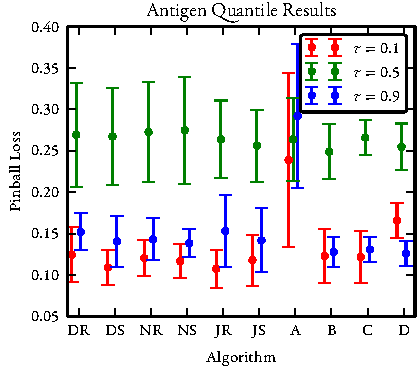
\includegraphics[width=\textwidth]{figures/Antigen_results}
		\end{subfigure}
		\begin{subfigure}[b]{0.32\textwidth}
			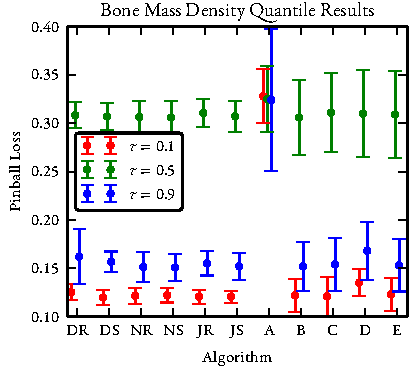
\includegraphics[width=\textwidth]{figures/Bone_Mass_Density_results}
		\end{subfigure}
		\begin{subfigure}[b]{0.32\textwidth}
			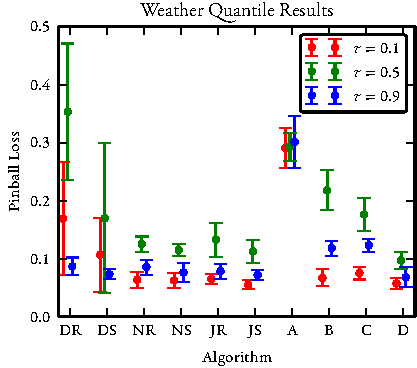
\includegraphics[width=\textwidth]{figures/Weather_results}
		\end{subfigure}
		\caption{Results from the three quantile experiments. The error bars in these figures represent $\pm 1$ standard deviation of the pinball loss over the testing set. A: Linear Quantile Estimator; B: Quantile SVM; C: Reduction to Classification; D: Quantile GP; E: Heteroskedastic Quantile GP}
		\label{fig:qfull}
	\end{figure*}
	% Suppose some data $\{(\bvec{y}_{i}, x_{i})\}_{i = 1}^{n}$ is collected from a joint distribution $\mathbb{P}_{\rv{Y} \rv{X}}$. We can either find the standard empirical embedding $\hat{\mu}_{\rv{X}}$ or empirical conditional embedding $\hat{\mu}_{\rv{X} | \bvec{\rv{Y}} = \bvec{y}}$, both of which is of the form $\Phi \bm{\beta}$. This is also true for posterior embeddings obtained from KBR \citep{fukumizu2013kernel}, making these techniques very general in nature.
	We present the following algorithms for quantile regression based on the methods proposed in this paper. Table \ref{table:quantile_regression_methods} lists the properties of each of these algorithms.

	\theoremstyle{definition}
	\begin{definition}
		Motivated by \cref{thm:empirical_distribution_and_cdf}, the \textit{direct embedding $\tau$-quantile estimate} (DR) is
		\begin{equation}
		q_{\rv{X}}(\tau) = \min\{x \in \mathbb{R} : \frac{1}{\sum_{i = 1}^{n} \beta_{i}} \sum_{i : x_{i} \leq x} \beta_{i} \geq \tau\}.
		\end{equation}	
	\end{definition}
	
	\theoremstyle{definition}
	\begin{definition}
		Motivated by \cref{thm:smooth_empirical_distribution_and_cdf}, the \textit{smooth embedding $\tau$-quantile estimate} (DS) is
		\begin{equation}
		q_{\rv{X}}(\tau) = x : \frac{1}{\int_{\mathbb{R}} k(0, x) dx \sum_{i = 1}^{n} \beta_{i}} \bm{\beta}^{T} \bvec{K}(x) = \tau.
		\end{equation}	
	\end{definition}
	
	For both approaches, pinball learning with cross-validation is used to optimise the hyperparameters. The normalisation factors ensure that the CDF approaches one as its input approaches infinity, and $k$ is assumed to be a stationary kernel.

	\theoremstyle{definition}
	\begin{definition}
		Using \eqref{eq:qpi_empirical_cdf} directly, the \textit{pre-image $\tau$-quantile estimate} is
		\begin{equation}
			q_{\rv{X}}(\tau) = x : \bvec{w}^{T} \bvec{K}(x) = \tau,
		\end{equation}	
		where $\bvec{w}$ is are the recovered density weights from QPI.
		We denote this algorithm as JB and JL when learned under pinball loss and marginal likelihood respectively.
	\end{definition}
	
	Since obtaining the density weights through \qpi\space requires a separate optimisation loop, this increases the time complexity of the algorithm significantly (see \cref{table:quantile_regression_methods}). At the expense of accuracy, the density weights can be instead obtained through clipping the embedding weights at zero and normalising them such that the resulting weights are valid PDF weights. For more detail, see the supplementary material. We then replace $\bvec{w}$ with these new and cheaply computable weights $\bvec{\tilde{w}}$ in \eqref{eq:qpi_empirical_distribution} and \eqref{eq:qpi_empirical_cdf}.
% * <lachlan@mccalman.info> 2016-10-06T00:07:22.658Z:
%
% There's a fukumizu paper I cite for this clipping process in my chapter 3 (can't remember now). Probably worth citing here.
%
% ^.

	\theoremstyle{definition}
	\begin{definition}
		The \textit{clip-normalised $\tau$-quantile estimate} is
		\begin{equation}
			q_{\rv{X}}(\tau) = x : \bvec{\tilde{w}}^{T} \bvec{K}(x) = \tau.
		\end{equation}
		where $\bvec{\tilde{w}}$ is the clip-normalised weights of the relevant embedding.
		Both pinball learning and marginal likelihood learning can be used. We denote this algorithm as NB when done with pinball learning, and NL when done with marginal likelihood learning.
	\end{definition}	
	
	\begin{table}[t!]
% * <lachlan@mccalman.info> 2016-10-06T00:07:58.096Z:
% 
% If you want to double check these complexity bounds I'd appreciate it  =)
% They make sense to me too
% 
% ^.
		\begin{center}
			\begin{tabular}{l|cccc}
				Algorithm & S & ND &   NC & Complexity \\ \hline
				DR  &              &                &                & $O(n \log(n))$    \\
				DS  & $\checkmark$ &                &                &
				$O(n \log(n))$  \\
				NB  & $\checkmark$ & $\checkmark$   &                &
				$O(n \log(n))$ \\
				JB  & $\checkmark$ & $\checkmark$   &                &
				$O(n^{3} \log(n))$ \\
				NL  & $\checkmark$ & $\checkmark$   & $\checkmark$   &
				$O(n \log(n))$ \\
				JL  & $\checkmark$ & $\checkmark$   & $\checkmark$   &   $O(n^{3} \log(n))$ 
			\end{tabular}
		\end{center}
		\caption{\small Comparison of Quantile estimation techniques. S stands for Smooth, ND for Non-Decreasing, NC for Non-Crossing, and $n$ is the number of training points.}
		\label{table:quantile_regression_methods}
	\end{table}
	
%	\subsection{Computational Complexity}
%	\label{sec:quantile_regression_algorithms:computational_complexity}
		
	The computational complexity of these algorithms varies from $O(n \log(n))$ to $O(n^{3} \log(n))$ in the number of training points $n$ (\cref{table:quantile_regression_methods}). The 1-D root-finding required to solve the quantile equation \eqref{eq:quantile_root_finding} introduces a factor of $\log(n)$ in all cases (using a binary search). The difference lies in the CDF estimation technique. %, whose computational complexity is discussed in the supplementary material.
	
	The cheapest algorithm is DR, which is simply a (conditional) sum of the mixture weights and is therefore $O(n)$ in the number of training points. Similarly, DS, NL, and NB are also $O(n)$, but requires pre-computation of the kernel integral $\eqref{eq:kernel_integral}$ of constant complexity. The most expensive are the \qpi-based pre-image estimators (JL and JB), which require solving a quadratic program and therefore introduces a further factor of $O(n^2)$. However, if a pre-image estimate is also required for other tasks and is therefore already available, then JL and JB also only introduces a further factor of $O(n)$.
	
\section{RELATED WORK}
\label{sec:related_work}

	Quantile regression was first introduced by \cite{koenker1978regression}, which considered inference based on an unknown linear model. Being more robust to noise and thus effective in modelling non-Gaussian behaviour, the median (0.5-quantile) is examined, rather than the mean. The Linear Quantile Estimator (Algorithm A) was constructed through minimising the pinball loss \eqref{eq:pinball_loss}, which, for a linear model, can be formulated as a linear programming problem with efficient solutions.
	
%	
%	The pursuit of conditional quantiles quickly divided the field into so-called direct methods, that attempt to directly compute the quantile from the training data through minimisation of the pinball loss, and Pre-Image methods, that attempt to first model the conditional cumulative distribution, and from there derive quantile estimates \citep{koenker2005quantile}.
%	
%	The direct initially demonstrated the advantage of flexibility --- nonparametric function estimation techniques could be applied that made no assumptions about the underlying distribution. Examples include locally-constant and locally-linear approximations \citep{Chaudhuri1991, Yu1998}. However, this flexibility also led to problems such as quantile crossing; in which a data point might be considered to be below the 0.5 quantile but above the 0.6 quantile \citep{koenker2005quantile}. 
%	
%	An important development was the addition of non-crossing constraints to direct quantile regression solutions \citep{He1997}. This ensured that different quantile estimates obeyed a strict ordering, with no two quantiles having the same function value. Such a strict ordering was achieved by adding a penalty term to the optimisation \citep{Cole1992}, or by reducing the class of possible functions used to represent the quantiles, for instance to classes of location-scale models \citep{Koenker1984, He1997}. Unfortunately, such models implicitly restricted the underlying distribution, causing reduced applicability to data that did not fit the assumptions of the model \citep{koenker2005quantile}.
%	
	\cite{takeuchi2006nonparametric} then examined Quantile SVM (Algorithm B), a conditional quantile estimation technique using support vector machines (SVM), which finds the decision boundary associated with the minimisation of the pinball loss and non-crossing constraints. However, such constraints may cause the resulting estimates to violate \cref{def:quantile} of a quantile.
%	
%	More recently, Chernozhukov et. al. developed a monotisation procedure based on function re-arrangement to remove crossing from quantile estimates generated by other algorithms. The resulting quantiles were guaranteed to be more accurate, and no assumptions were made about the underlying distribution \citep{Chernozhukov2010}.
%	

	Other direct approaches include the `quanting' algorithm \citep{langford2012predicting}, or Reduction to Classification (Algorithm C), which re-casts the quantile regression problem as a classification problem. By placing a set of classifiers over the range of the regression, each classifier can be trained on whether the quantile is above or below it. The quantile estimate is then the expectation of this assignment, over all the classifiers.

	Pre-image techniques for conditional quantile regression have also been examined in the semi-parametric and nonparametric setting. \cite{yu2001bayesian} used a parametric linear model with Laplacian likelihood and uniform prior, which makes the unimodal assumption, and requires Markov chain Monte Carlo (MCMC) integration for inference. Similar semi-parametric methods such as \cite{hjort2007nonparametric, hjort2009quantile} use Dirichlet process priors, which again requires costly inference approximations.
	
	In the nonparametric setting, \cite{quadrianto2009kernel} examined kernel conditional Quantile GP (Algorithm D) using Gaussian process regression (GPR) to explicitly compute the resulting CDF, for which analytical forms exist. The Gaussian structure enforces non-crossing constraints and allows for efficient inference. Additionally, heteroskedastic covariance functions were employed to account for input-dependent noise in the data, leading to Heteroskedastic Quantile GP (Algorithm E). However, while nonparametric and Bayesian, the Gaussian structure restricts applicability to symmetric, unimodal phenomenon.
	
	\cite{boukouvalas2012gaussian} then extends this GPR framework by instead minimising the expected pinball loss \eqref{eq:pinball_loss}, so that the technique is specifically optimised for obtaining quantiles. The resulting learning algorithm then loses its analytical tractability, and is computed by expectation propagation instead. With a similar goal, \cite{abeywardana2015variational} instead replaces the Gaussian likelihood involved in GPR with a scaled exponentiation of the pinball loss \eqref{eq:pinball_loss}, and uses variational inference to approximate the resulting intractable posterior, leading to a powerful and flexible quantile regression framework. However, while asymmetric, the likelihood is still unimodal, again limiting its capability to model multimodal phenomenon.
	 
%	A more general formulation of Bayesian quantile regression was developed in \cite{taddy2012bayesian}, which used Dirichlet process mixture models to represent the underlying joint distribution. This allowed a very general class of distributions to be represented, but inference required expensive MCMC integration.
	
	To overcome the limitations of these methods, we apply kernel embedding techniques to represent general probability distributions nonparametrically. Without limiting the resulting distribution to any particular parametric form, quantile regression with kernel embeddings can model a variety of phenomenon which exhibits various structural forms.
	
% * <lachlan@mccalman.info> 2016-10-06T00:09:48.133Z:
% 
% Any luck finding a few recent citations for the related work section? Maybe check who has cited some of these papers cerently. Particalrly quadrianto2009kernel
% Kelvin: Yes! I should have included abeywardana2015variational, which is also one of Fabio's papers. I will do that now.
% Done.
% 
% ^.
	

	
\section{EXPERIMENTS}
\label{sec:experiments}
		
	We now test the performance of our algorithms on four standard datasets commonly used in the literature for conditional quantile estimation: Antigen, Weather, Bone Mineral Density, and Motorcycle. Antigen, Weather and Motorcycle were taken from the UCI repository \citep{lichman2013uci} and Bone Mass Density from the ``ElemStatLearn'' R package \citep{hastie2005the}. We compare our algorithms to state-of-the-art direct and pre-image techniques for conditional quantile estimation (Algorithms A, B, C, D, and E).
	
%	We now test the performance of our quantile estimators on a number of standard machine learning datasets. We compare our algorithms to state-of-the-art direct and pre-image techniques for conditional quantile estimation from the literature (Algorithms A, B, C, D, and E). % These include Linear Quantile Estimation (A) \citep{koenker1978regression}, Quantile SVM (B) \citep{takeuchi2006nonparametric}, Reduction to Classification (C) \citep{langford2012predicting}, Quantile GP (D) \citep{quadrianto2009kernel}, and Heteroskedastic Quantile GP (E) \citep{quadrianto2009kernel}.
%	
%	We evaluated the algorithms on four datasets commonly used in the literature for conditional quantile estimation tests: Antigen, Weather, Bone Mineral Density, and Motorcycle. Antigen, Weather and Motorcycle were taken from the UCI repository \citep{lichman2013uci} and Bone Mass Density from the ``ElemStatLearn'' R package \citep{hastie2005the}.
	
	For all experiments, performance was evaluated by five-fold cross validation and the average pinball loss over the hold-out set. The average, and standard deviation, of the performance over these five tests was used as the final score. Three quantile levels $\tau$ were tested for each dataset: 0.1, 0.5 and 0.9. Any categorical variables in the data were ignored. All input and output variables were standardised to have zero mean and unit variance in each dimension.
	
	We place a Gaussian kernel for both the input variable $y$ and the output variable $x$. For the input $y$, we whiten the data to decorrelate each dimension using a form of automatic relevance determination \citep{rasmussen2006gaussian} such that an anisotropic but diagonal Gaussian kernel can be used. All our algorithms were trained with (nested) five-fold cross-validation.
% * <lachlan@mccalman.info> 2016-10-06T00:13:07.395Z:
%
% These were standard datasets when I did this work, hopefully someone has done something recently we can add here? 
%
% ^.
	\subsection{Results}
	\label{sec:experiments:results}
		
% * <lachlan@mccalman.info> 2016-10-06T00:12:22.660Z:
%
% I don't know what fabio would think about this, but could we put the full results table in the sup material? 
% Done.
		
		The average pinball loss for each algorithm in the three experiments is given in \cref{fig:qfull}. Overall, pre-image algorithms performed on par or better than algorithms from the literature. The two best performing algorithms were NB and JB, which are the normed-weights and \qpi\space methods, trained under the pinball loss. % It is unsurprising that pinball learning performed better than marginal likelihood learning, given that the training was optimising the same function that would evaluate the algorithm's performance.

		This demonstrates a trade-off between using pinball learning and receiving slightly better performance, or marginal likelihood learning (NL and JL) and ensuring the non-crossing constraint holds. % The NL and JL algorithms were competitive, but kernel conditional Quantile GP (D) achieved the best performance.

		With both pinball and marginal likelihood learning, there was little difference on average between the pre-image estimator and the normed-weights estimator. This fact is worth noting when considering a real-time application of these algorithms, as the pre-image estimator has a much greater computational cost.
		
		Over the three experiments, we see that extremal quantiles 0.1 and 0.9 have significantly lower pinball loss compared to the median (0.5). There appear to be no algorithm that is especially capable at a particular quantile, although two direct methods (DR and DS) are much more competitive at the extremes than the median. Intuitively, an accurate estimate of the median is affected by nearby observations both above and below it. However, direct methods only sum contributions from points below the median, while pre-image methods considers all mixture components. Far away from the median, there are fewer points nearby, reducing this effect on direct methods.
		
%		The likely explanation is that, in general, an accurate (empirical) estimate of the median is affected by nearby points both above and below it. These direct methods however only sum contributions from points lying below the median. The pre-image methods on the other hand, sum contributions from mixture components centred at all training points. Far away from the median, there are fewer points nearby and so the effect is reduced.
		
		\begin{figure}[t]
			\begin{center}
				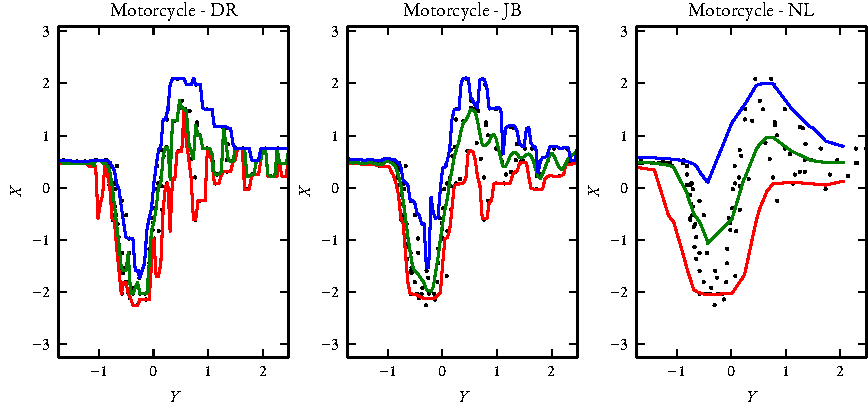
\includegraphics[width=\columnwidth]{figures/mcquantilesall}\\
			\end{center}
			\caption{Examples of 0.1 (red), 0.5 (green) and 0.9 (blue) quantile estimates for the Motorcycle dataset, for the DR, JB, and NL algorithms.}
			\label{fig:motorcycleresults} 
		\end{figure}
		
		Figure \ref{fig:motorcycleresults} plots the quantiles estimated for the Motorcycle dataset for three of the algorithms. The piecewise-constant quantile estimates are clearly visible in the DR plot. The JB plot has each quantile trained separately, and as a result the 0.1 and 0.9 quantile both fit the boundary of the data very closely. The NL plot shows a much smoother representation, as these are quantiles for a single underlying cumulative distribution (trained with the marginal likelihood learning).

\section{CONCLUSION}
\label{sec:conclusion}
	
	This paper presented a set of novel algorithms for estimating quantiles nonparametrically from kernel embeddings of probability distributions given sampled observations. By projecting indicator functions into the RKHS spanned by features at the observations, we first present an efficient direct non-smooth CDF estimate. We then impose smoothness by instead projecting a smooth function into the full RKHS. At a trade off with computational complexity, the non-decreasing constraint is then guaranteed by a pre-image approach, where the effective weights is to be recovered from a quadratic program.
	
	We then construct quantile estimators from these CDF estimates using numerical root-finding, and considered training on both the pinball loss and the log marginal likelihood. Finally, the resulting algorithms are tested on a set of well-known machine learning datasets.
	
	Our pre-image quantile estimators in particular were comparable to, or better than, state-of-the-art algorithms. These algorithms can be trained either using pinball loss, for a slight increase in performance, or with negative log marginal likelihood, to guarantee the non-crossing constraint. Additionally, all our algorithms explicitly represent multimodal distributions, and can model datasets with strong heteroskedasticty.
	
	An interesting direction for future work would include the investigation of a complete Bayesian learning framework, where the latent phenomenon can be represented as a kernel embedding, and the learning objective is evaluated over the whole training set at once instead of over a separate validation set, similar to marginal likelihood learning in the GPR framework.

%\section*{Acknowledgements}
%
%	This work is supported by anonymous organisations.

\newpage
\bibliography{kernel_embeddings}

\end{document}
